\section{Methods}
In this section, we report the results of multiple methods we tried for feature extraction, dimension reduction, and classification. 


\subsection{Dimensionality Reduction}
\subsubsection{Feature Selection Using Information Gain and Bi-normal Separation}
To extract informative features from the raw word and image features,  we first ranked words features by based on their Information Gain (IG) and Bi-normal Separation (BNS), below is the comparison of the top 30 words selected by IG and BNS.   
\begin{center}
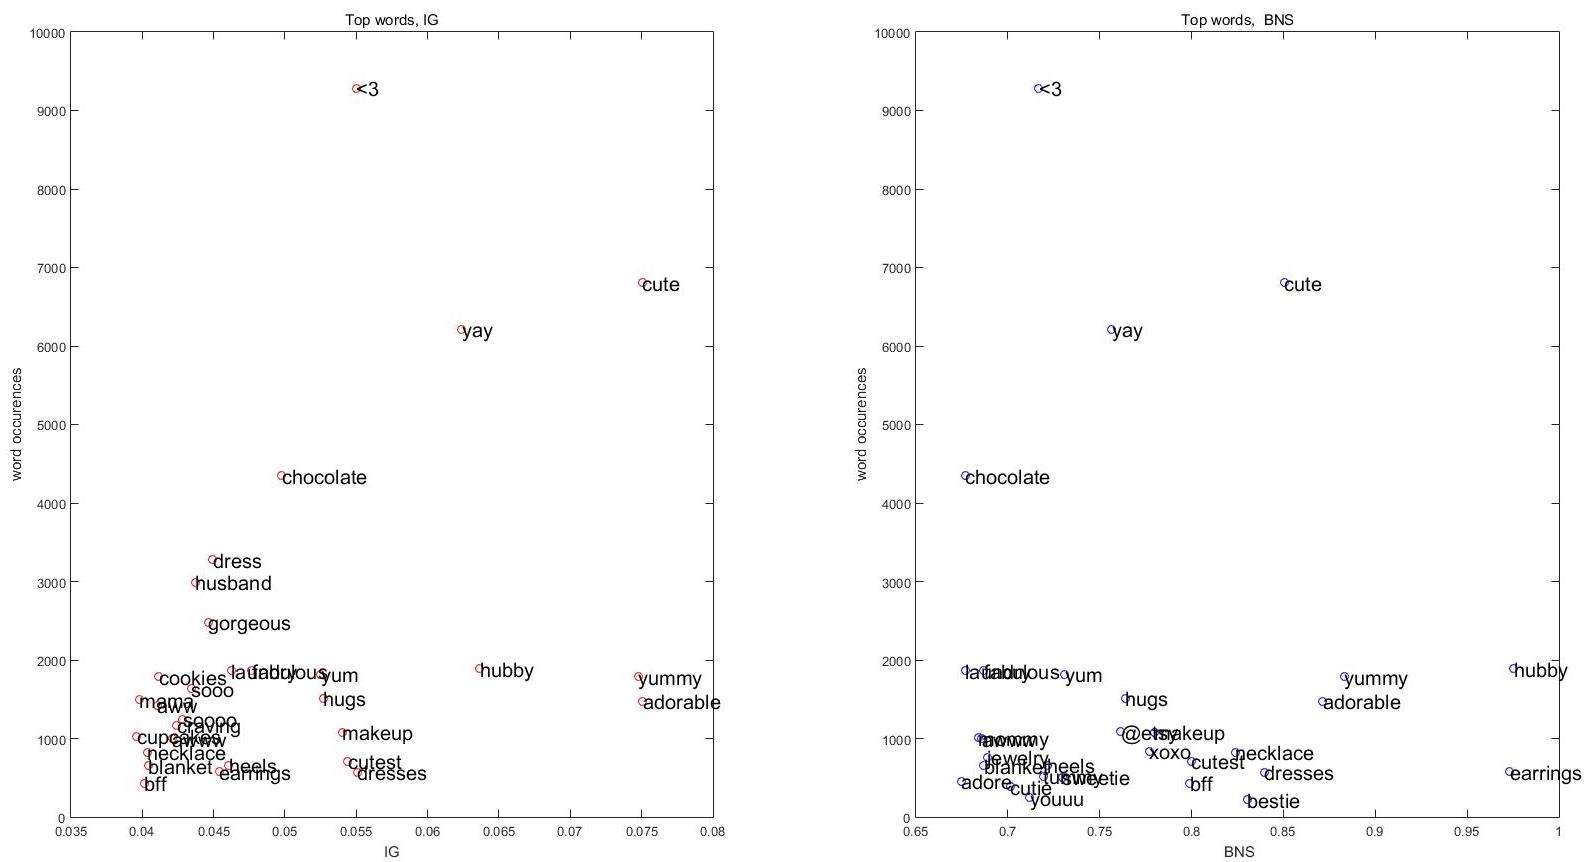
\includegraphics[scale=0.30]{topwords.jpg}
    \end{center}
Next we examine the frequency of the top 1000 words selected by IG and BNS. Each circle in the graph below represents one word.
\begin{center}
    \fbox{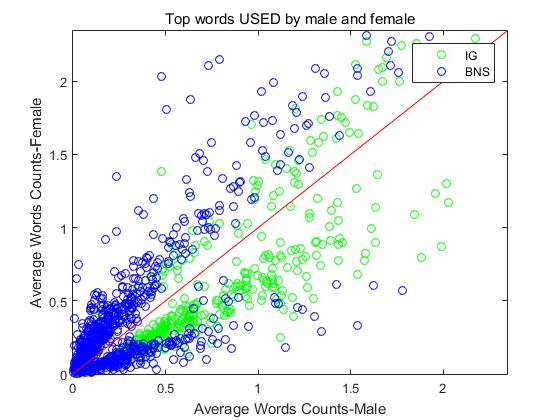
\includegraphics[scale=0.40]{topwordsB.jpg}}   
    % \hspace{30px}
    \fbox{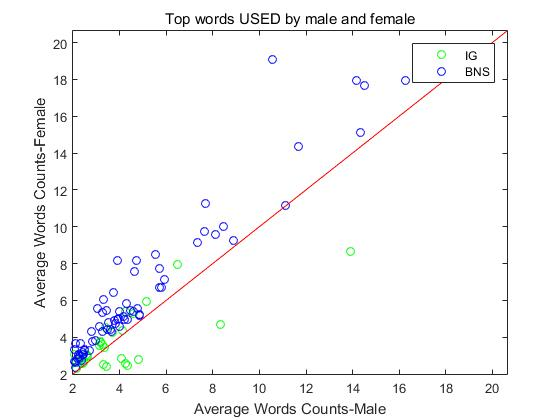
\includegraphics[scale=0.40]{topwordsC.jpg}}
    % \hspace{30px}
\end{center}
% \begin{center}
% 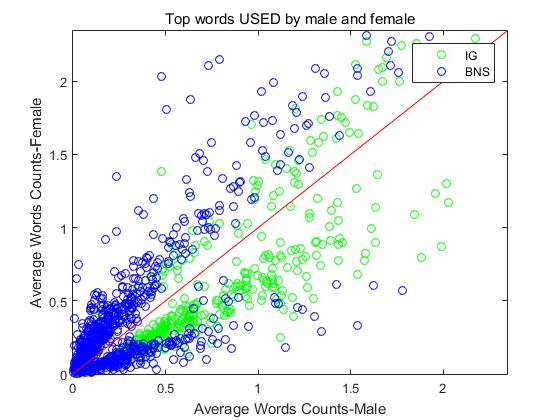
\includegraphics[scale=0.5]{topwordsB.jpg}
% \end{center}
When the average words counts is less than 2.5, BNS selects the words that are more frequently used by either male or female.\\
% \begin{center}
% 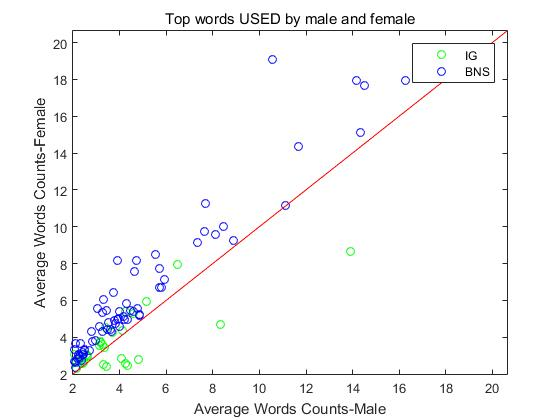
\includegraphics[scale=0.5]{topwordsC.jpg}
% \end{center}
Furthermore BNS tend to select more high frequency words used by female.\\
Finally, we test the effectiveness of the two feature selection methods by examining the improvement on cross validation accuracy over the following models: Logitboost with stump trees, logistic regression and naive bayes.
BNS works well on Naive Bayes (though we didn't include this model in our final submission); IG improves the accuracy of Logitboosting with decision stump trees, no feature selection works better for logistic regression with L2 regularization on words.\\
\subsubsection{PCA}
We used PCA on both words and images feature. In this project, we found that PCA works relatively well on image features but not as good on words features. The details will be discussed with the following sections.
%\subsubsection{Stemming and Stop Words}
%We tried to do stemming and removal of the stop %words on words features. However, in this project, %we found it not so helpful.

\subsection{Classification on Tweets}

\subsubsection{Logistic Regression on Raw Words and Extracted Image Features}
Since the project is a binary classification task. logistic regression might be a good choice for the first try. We first put PCA-ed words features and extracted images features into logistic regression with l2 regularization for training and classification, which beat baseline 1 with 86.01\% accuracy. We later tried just use raw words features without extracted image features, which surprisingly, obtained 86.83\% accuracy. 
\subsubsection{Neural Network}
We employed 4 layers neural network (5000-100-50-2). We trained neural network 200 epochs with decreasing learning rate. For every 50 epochs, we decreased the learning rate to one-tenth of the last. The neural network produced around 86\% accuracy on words features.
\subsubsection{Logitboost with Stump Trees}
Logitboost can be seen as a convex optimization which combines Adaboost with the cost function of logistic regression, which is suitable for binary classification. Using this model, our team acheives a tesing accuracy of 89.11\%. More details will be discussed in \ref{logitboostFSIG}.
\subsubsection{SVM with Intersection Kernel}
We trained two SVMs with Intersection Kernel on the top 1000 words+image features ranked by information gain. One model is trained on the original data and the other is trained on L2 normalized data. The former gives a cross validation accuracy of 87.10\% and the latter gives 88.68\%. More details please refer to \ref{kernelsvmensemble}.\\
\subsection{Images Features Extraction and Classification}
\subsubsection{Grey-scale Images}
We first converted the profile images data into R, G, B and Grey-scale images. 
\subsubsection{Face Detection with Viola-Jones Algorithm}
We extracted all the faces. We used matlab built-in Viola-Jones algorithm to do face detection on RGB images, which detected faces on 72\% of the profile pictures. All the following classifications over images were based on the faces detected. Later when ensemble, we only used samples with detected faces. For those samples without faces in them, we just set the output of the classifier as 0 (the output of the classifier is either positive or negative for male or female).
\subsubsection{Logistic Regression with Eigen Faces}
After extracted faces, we did PCA over grey-scale images, the visualization of the top principal components are shown in figure below. We put top PCs into logistic regression classifier and it yielded around 70\% accuracy over detected faces. \\
\begin{center}
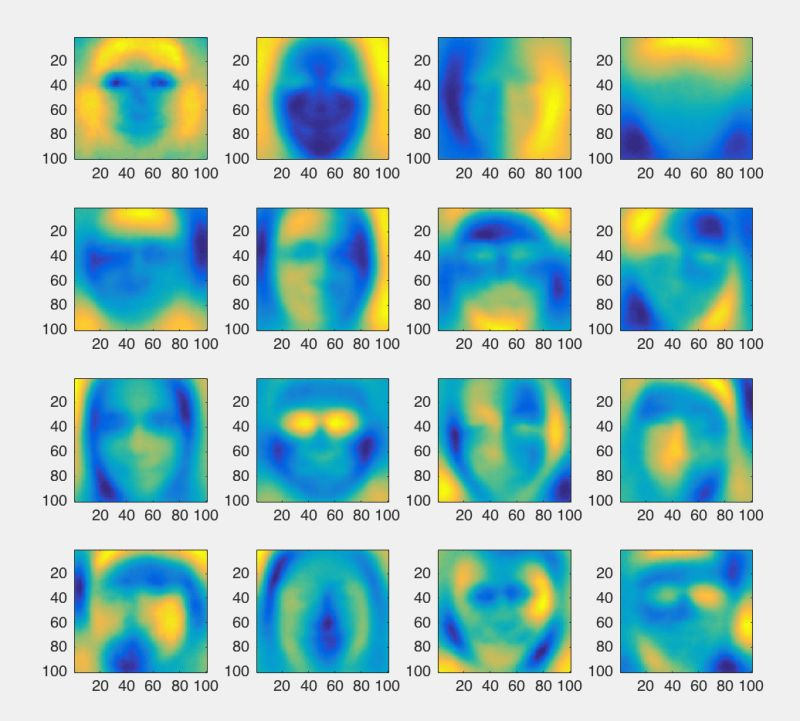
\includegraphics[scale=0.5]{pca_faces}
\end{center}
\subsubsection{HOG Features, Gaussian Pyramid, Eyes and Nose}
We used Viola-Jones algorithm to detect and crop eyes and nose. After that, we extracted Gaussian Pyramid HOG features on faces, eyes and nose into 7020 feature vector. Classifying the features with logistic regression yielded 82\% accuracy by itself on 72\% detected faces. The ensemble with this classifier produced 91.9\% over all accuracy on the test set. 
\subsubsection{SVM on PCA-ed HOG Features}
We then replaced the logistic regression classifier with a more powerful RBF kernel SVM. The accuracy on detected faces was improved up to 83\%. The ensemble with this classifier got 92.3\% accuracy on the test set.  Then we did PCA (1500 PCs) on HOG features to reduce the dimensionality and the size of SVM model. The accuracy of the single model with improved to 84\%. However, the ensemble with this classifier dropped to 92.14\% accuracy on the test set. 
\subsubsection{SVM on PCA-ed Dense LBP Features}
LBP works complementary with HOG features, we extracted spatial pyramid LBP features (15871 features) on detected faces and trained a SVM classifier over 2000 principal components of the LBP features. This model achieved 85\% accuracy on detected faces. We integrated this model to the ensemble yielded our highest accuracy on the leaderboard of 92.42\% on test set.

\subsubsection{Auto-encoder}
The Auto-encoder was employed for image dimensionality reduction on Grey-scale face images we detected and extracted. We experimented with various neural network settings and found the optimal number of hidden nodes is 100. We also set the learning rate to be 0.5, input zero-masked fraction to be 0.8, scaling-learning rate to be 0.95, non-sparsity penalty to be 0.1, and drop-out fraction to be 0.25. Our cross-validation using logistic regression shows over 75\% accuracy on the face-detected images.
The visualization of the auto-encoder is shown below. 
\begin{center}
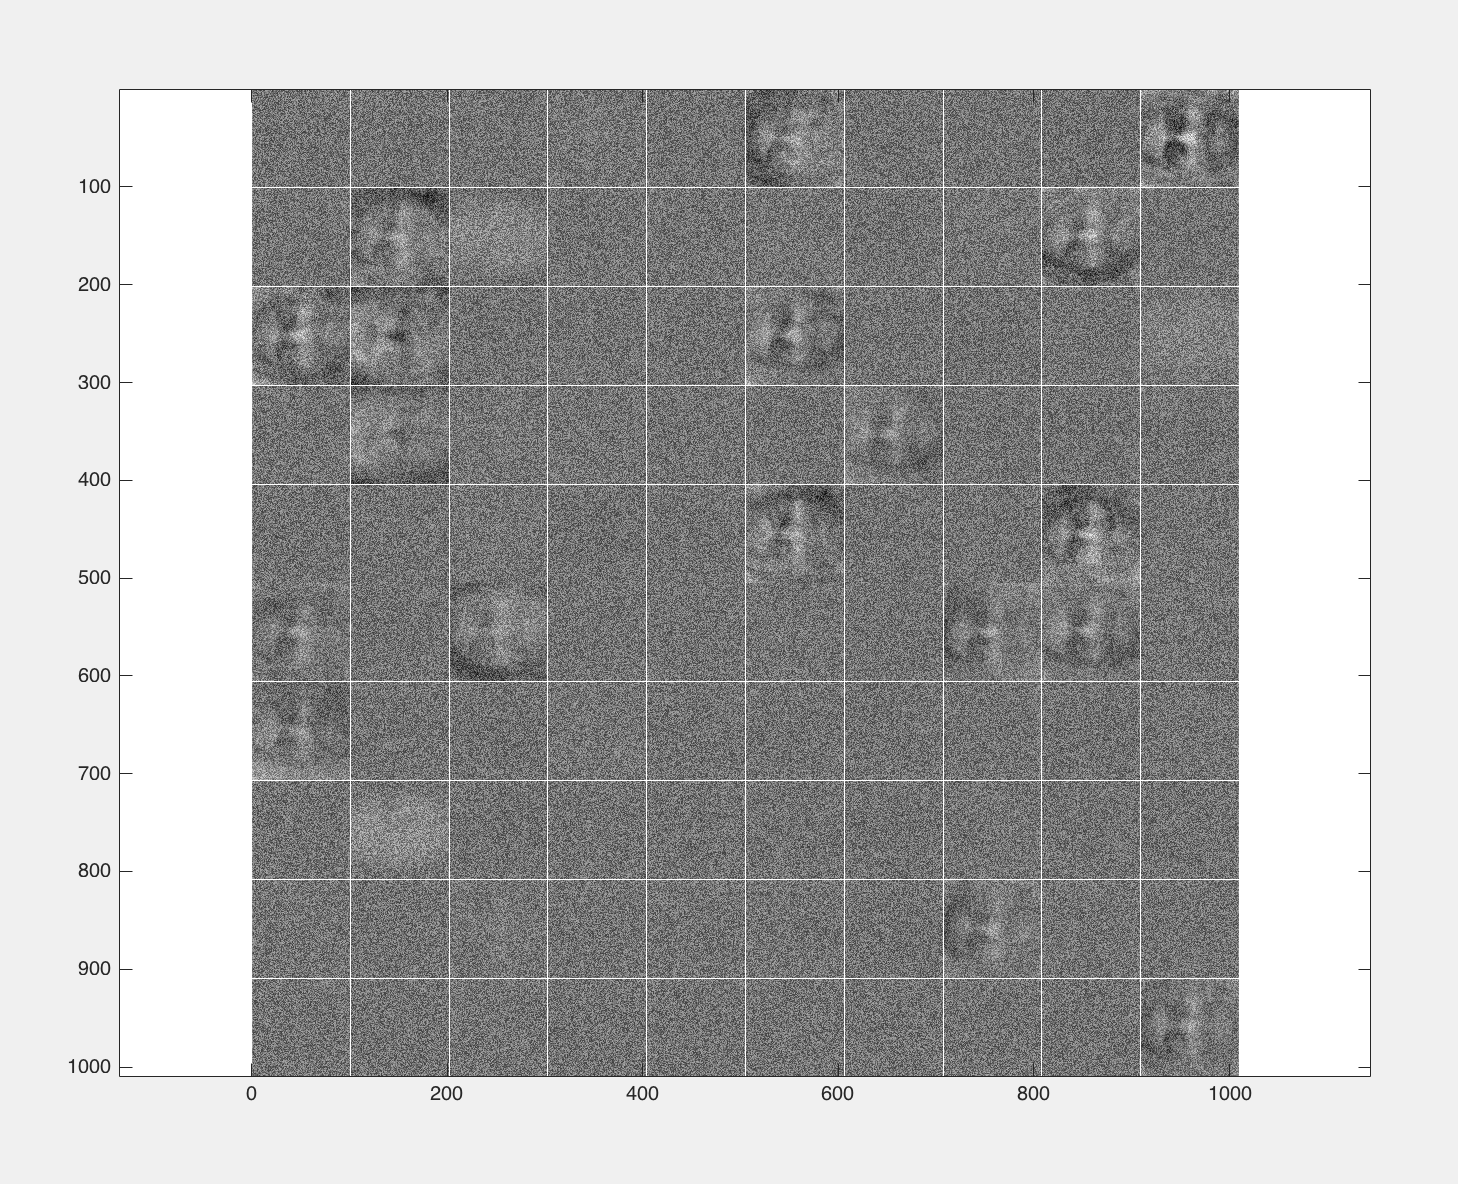
\includegraphics[scale=0.45]{autoencoder.png}
\end{center}
\subsection{Ensemble Methods}
\subsubsection{Stacking}
We used stacking to ensemble our models to achieve better over all performance than any of the single models. First, we used 80\% of the training data to train all the single models including logistic regression, neural network, logitboost with feature selection, kernel SVM with feature selection, kernel SVM with normalization, SVM over PCA-ed HOG, SVM over PCA-ed LBP. And then, use those models to generate scores (raw outputs) for the rest 20\% data. Training a logistic regression model using the 20\% scores with labels yields a ensemble classifier. Finally, we use all the training data to re-train all the single models. Along with the ensemble classifier, we got our final model. 
\subsubsection{Normalization}
When ensemble all the models, we noticed that normalization actually works. For the images, we first trained logistic regression on raw gaussian pyramid HOG features (faces, eyes and nose), which yielded 82\% accuracy on detected faces by itself. Later, we figured SVM works better by experiment (84\%). However, when we ensemble the new model, it actually produced lower accuracy. We then found that the scores ranges produced by logistic regression and SVM were actually different. This may cause unbalanced weights across models. We then normalized all the scores with a sigmoid function with mean 0 and variance 2. This produced higher overall accuracy (92.3\%). 

\subsection{Final Submission}
Considering the time and space constraints, we finally submitted 5 models including logistic regression on words features, neural network, logitboost, kernel SVM and bagging of logistic regression models on HOG features. In this section, we analyze the over all performance of those 5 models.

\subsubsection{LogitBoost and Feature Selection Using Information Gain}
\label{logitboostFSIG}
 We want to use both words features and image features in order to enhance our accuracy, but we don't know which feature is most informative; therefore, we ranks all words and image features together using information gain and select the top features (In fact, by computing the information gain of image features, we found image feature 1 2 5 6 and 7 have roughly 0 information gain, but of course this does not mean all image features are useless).\\
On the other hand, Logitboost can be seen as a convex optimization which combines Adaboost with the cost function of logistic regression. We experiment with Logitboost based on the following considerations.\\
1. Words and the seven image features have different scales, we need a model that is scale invariant; boosting with decision stump trees in this case is a great choice.\\
2. The cost function using logistic regression is suitable for binary classification, it is a convex problem and minimizes the binomial deviance and gives less weights to misclassified observations.\\
By selecting the top 1000 features ranked by information gain and using 300 decision stump trees, we achieved an accuracy of 89.11 percent on the testing set.\\
In our final submission, this model also serves as a major classifier that contributes to our ensemble method.\\
Below is the cross validation accuracy plots (over 8 folds, with each curve represents one fold):\\
\begin{center}
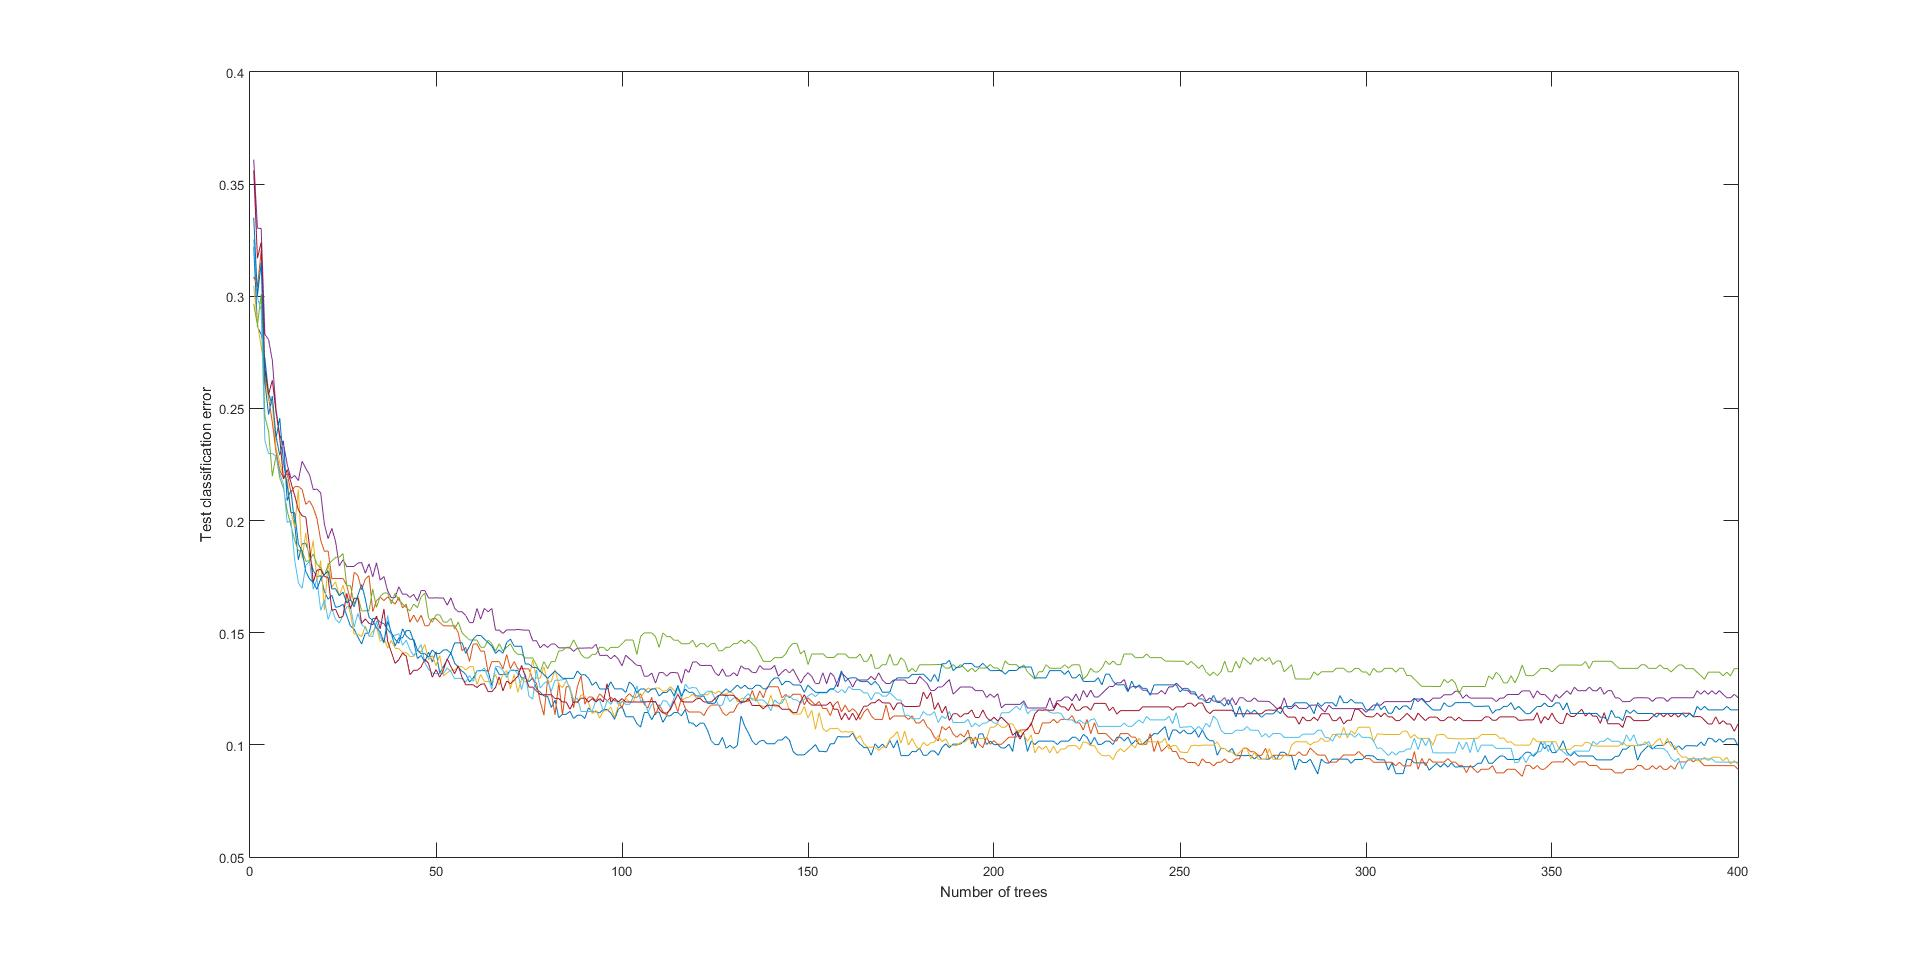
\includegraphics[scale=0.3]{logitboost.jpg}
\end{center}
\subsubsection{Kernel SVM for Ensemble}
\label{kernelsvmensemble}
The major motivation for introducing the Kernel SVM on words is to enhance our final ensemble accuracy. In order to do that, first we need to understand the contribution of each individual classifier to the ensemble. Below is the bar chart demonstration: (note when the ensembler only receives a single input, the outputs from Log-reg on words, our ensembler simply gives the predictions from the Log-reg classifier)\\
% \begin{center}
% 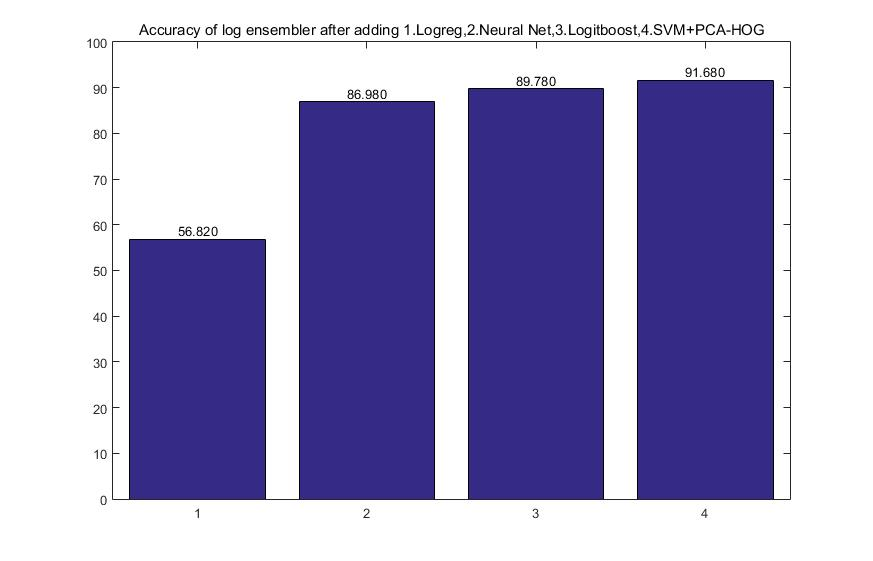
\includegraphics[scale=0.4]{ens_add_acc.jpg}
%     \end{center}
%\begin{figure}[!ht]
%  \caption{Ensemble with multiple classifiers}
%  \centering
%    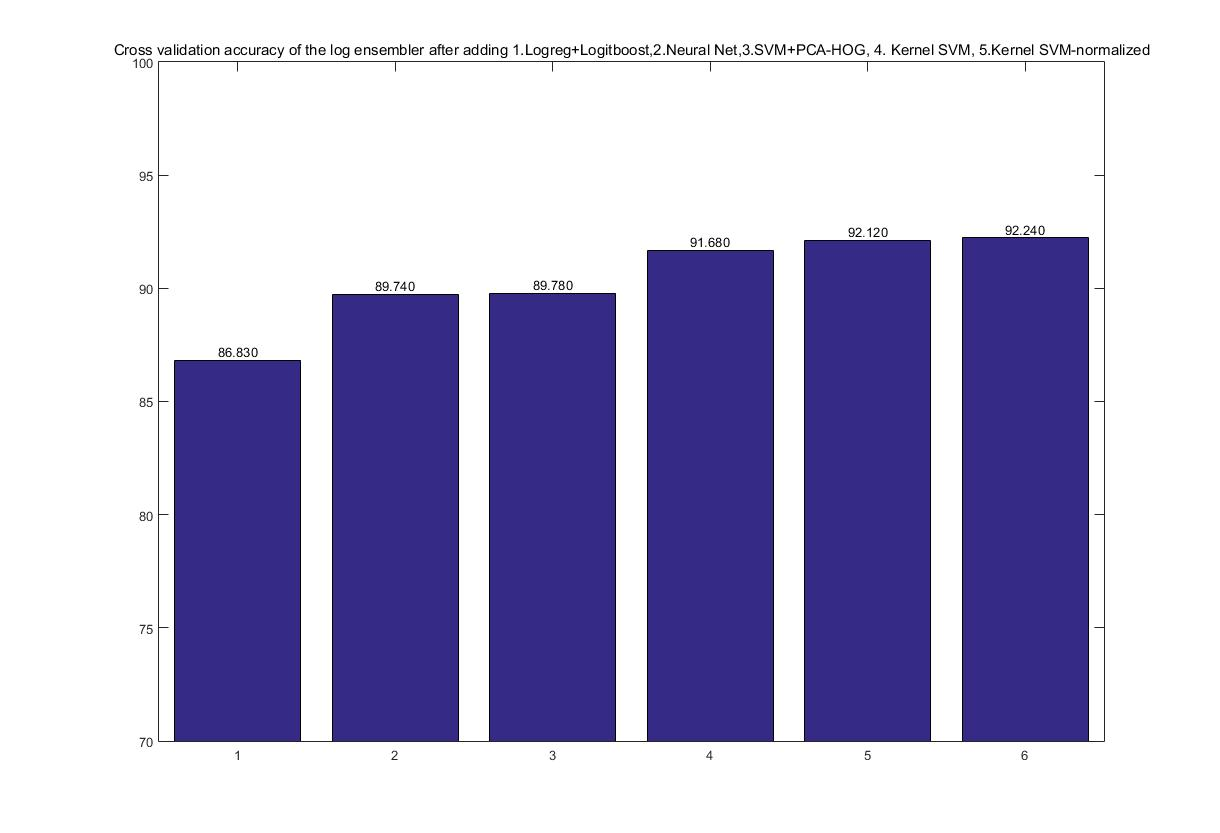
\includegraphics[width=1\textwidth]{ens_add_accB.jpg}
%\end{figure}
 \begin{center}
 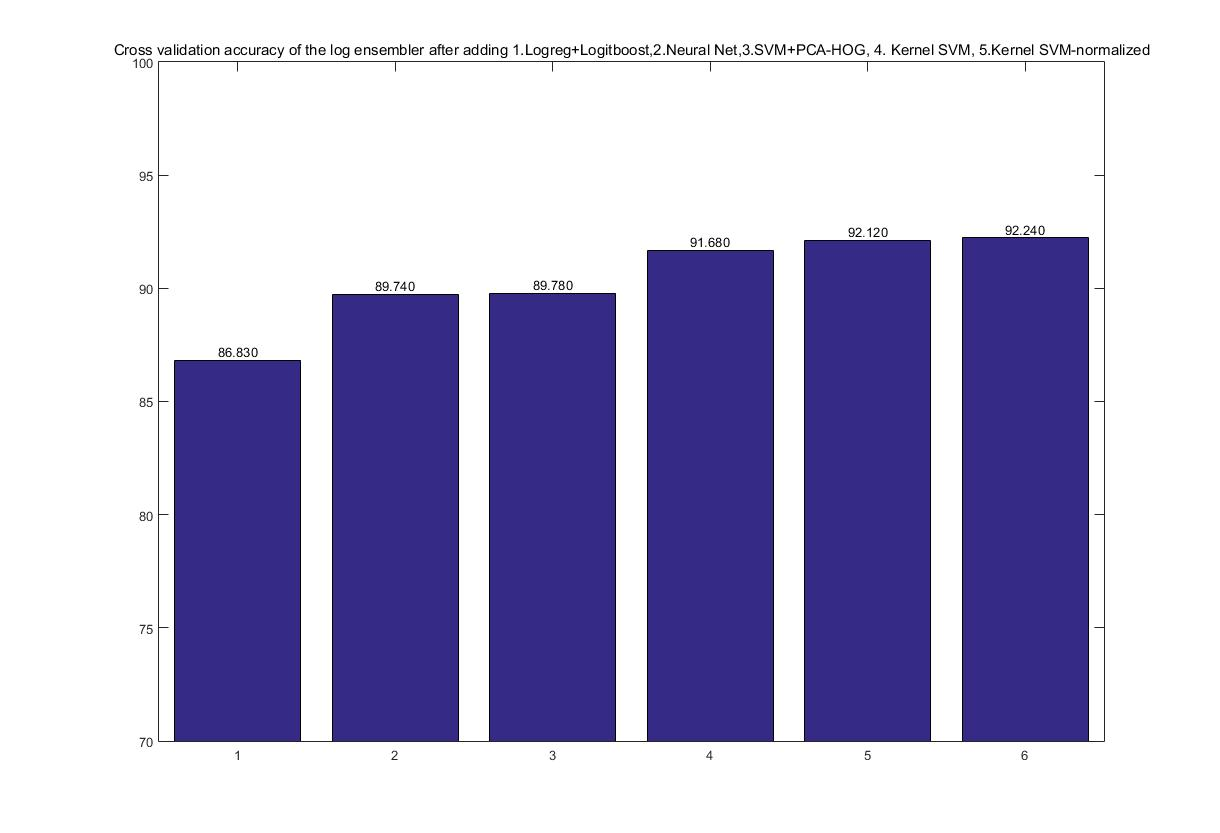
\includegraphics[scale=0.40]{ens_add_accB.jpg}
     \end{center}
For our kernel SVM on words and image features, the Intersection Kernel is used for investigating the interactions between features (which we haven't done in the former models), and feature intersection might be a good way to obtain information about feature interactions.\\
We trained two Kernel-SVM on the top 1000  features based on information gain from the image feature and words training set: one on the original set; the other on the L2 normalized version of the data. We keep both models since in reality it's hard to say which model is less useful. Our goal is to enhance to the accuracy of our ensemble; therefore each model may give different but still useful information in different aspects. The bar plot below shows the improvement after adding the two models. (Note: all cross validation are performed on the same cross validation sets (5 sets in total)). This is the last ensemble combination we proposed one day before the submission deadline and unfortunately we haven't got a chance to obtain the accuracy on the testing dataset.\\
% \begin{center}
% 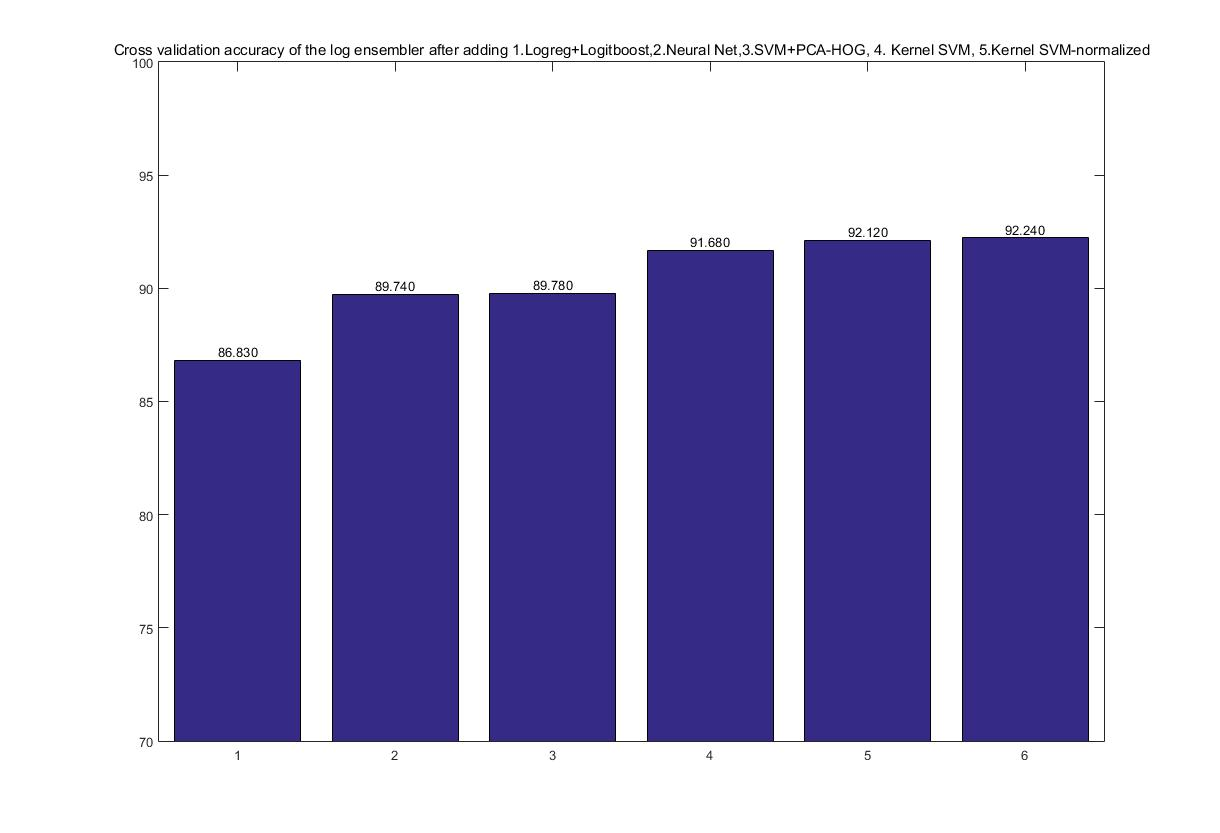
\includegraphics[scale=0.40]{ens_add_accB.jpg}
%     \end{center}

\subsubsection{Bagging Logistic Regression on Raw HOG Features}
To meet the time and space constraints of the competition, we dropped LBP model and and replaced the big SVM model with bagging logistic regression. Because the basis of PCs took 130Mb, which was too large for 50Mb space constraint, we didn't do PCA in the final submission either. Instead we used a bagging logistic regression with 6 logistic regression  models, with each of them trained on 60 percent randomly resampled data from the original dataset. Bagging is another ensembling method we experiemented for thie project. In short, it trans multiple models on different subsets of original dataset, by doing so the model variance and overfitting can be reduced. We investigated on the bagging of Naive Bayes and Logistic regression. Bagging doesn't show significant improvements on Naive Bayes (in the writer's optinion, this makes sense, as Naive Bayes is just a simple categorical statistical model, a sum of multiple such models can been viewed as a big Naive Bayes model), but for logistic regression, as shown in our project demo, it can increase the accuracy of logistic regression on words and image features from 86.83\% to 87.56\%, if correcly configured; on HOG features, it increases the cross validation accuracy from 78.53\% to 82.14\%.  After replacing SVM-HOG with baged logistic models, our cross validation accuracy dropped from 92.24\% to 91.36\%. The final model produced 91.04\% accuracy on validation set.

